\documentclass[11pt]{article}
\usepackage[margin=1in]{geometry}
\usepackage[T1]{fontenc}
\usepackage[utf8]{inputenc}
\usepackage{lmodern}
\usepackage{amsmath}
\usepackage{graphicx}
\usepackage{booktabs}
\usepackage[hidelinks]{hyperref}
\usepackage{microtype}
\usepackage[font=small,labelfont=bf]{caption}

% generated by paper/make_numbers.py from results/ -- do not edit
\newcommand{\Neurons}{156}
\newcommand{\Inputs}{116}
\newcommand{\NPFNa}{55}
\newcommand{\NPFNd}{40}
\newcommand{\NPFNv}{21}
\newcommand{\Intermediates}{14}
\newcommand{\NhDeltaA}{11}
\newcommand{\Outputs}{26}
\newcommand{\Edges}{2190}
\newcommand{\EdgesInMid}{87}
\newcommand{\EdgesMidOut}{70}
\newcommand{\EdgesWithinInputs}{1958}
\newcommand{\EdgesDirect}{0}
\newcommand{\NParams}{141}
\newcommand{\NSeeds}{5}
\newcommand{\TestGames}{100}
\newcommand{\BudgetFrames}{4{,}000{,}000}
\newcommand{\NGood}{4}
\newcommand{\NBad}{1}
\newcommand{\GoodWinPct}{100}
\newcommand{\GoodAgainstMin}{0.15}
\newcommand{\GoodAgainstMax}{0.95}
\newcommand{\GoodReturnMin}{96.2}
\newcommand{\BadFor}{5.55}
\newcommand{\BadAgainst}{10.89}
\newcommand{\BadWinPct}{4}
\newcommand{\BadSeed}{3}
\newcommand{\TrainTimeMean}{53}
\newcommand{\RuleFor}{1.74}
\newcommand{\RuleAgainst}{0.02}
\newcommand{\RuleWinPct}{62}
\newcommand{\StillFor}{3.12}
\newcommand{\StillAgainst}{10.99}
\newcommand{\RandFor}{1.54}
\newcommand{\RandAgainst}{11.00}
\newcommand{\DiagBaseFor}{0.59}
\newcommand{\DiagBaseAgainst}{11.00}
\newcommand{\DiagBestFor}{10.31}
\newcommand{\DiagBestAgainst}{5.66}
\newcommand{\MidLesForMax}{1.7}
\newcommand{\LesionRows}{intact & 11.0--0.9 & 11.0--0.6 & 10.8--0.2 & 5.5--10.9 & 11.0--0.1 \\ all intermediates ($h\Delta$) & 0.2--11.0 & 1.7--11.0 & 1.4--11.0 & 0.2--11.0 & 0.0--11.0 \\ all PFN inputs & 0.2--11.0 & 1.7--11.0 & 1.4--11.0 & 0.2--11.0 & 0.0--11.0 \\ PFL3 left & 10.7--7.0 & 10.7--6.7 & 9.7--7.5 & 0.3--11.0 & 0.1--11.0 \\ PFL3 right & 2.0--11.0 & 8.2--10.5 & 10.5--7.0 & 5.5--10.8 & 11.0--0.9 \\ DNa02 (both) & 11.0--1.8 & 11.0--1.6 & 9.1--1.1 & 5.3--10.9 & 10.7--0.9 \\}
\newcommand{\DiagRows}{base & 61 & 0.59--11.00 & 2.2 \\ rho0.5 & 61 & 1.00--11.00 & 3.6 \\ T8 & 61 & 0.19--11.00 & 1.0 \\ per-neuron readout & 85 & 8.88--9.88 & 21.1 \\ per-neuron readout, k\_in 16 & 141 & 10.31--5.66 & 26.7 \\}
\newcommand{\SeedRows}{0 & 11.00--0.95 & 100\% & 24.4 & 96.2\% & 52 \\ 1 & 11.00--0.55 & 100\% & 25.6 & 97.9\% & 56 \\ 2 & 10.84--0.19 & 100\% & 51.7 & 99.6\% & 52 \\ 3 & 5.55--10.89 & 4\% & 13.6 & 55.4\% & 53 \\ 4 & 10.99--0.15 & 100\% & 41.8 & 99.6\% & 54 \\}


\title{\textbf{Steering a Paddle with the Central Complex:\\a Connectome-Constrained Pong Agent}}
\author{Burak G\"ulmez\\[2pt]
\small College of Engineering and Architecture, University College Dublin, Dublin, Ireland\\
\small \texttt{burak.gulmez@ucd.ie}}
\date{}

\begin{document}
\maketitle

\begin{abstract}
\noindent
In the fly brain, an internal estimate of heading is converted into steering commands by the central
complex. A pathway of this region is isolated in the FlyWire reconstruction (\Neurons{} neurons and
\Edges{} connections, running from PFN columnar cells through h$\Delta$ interneurons to PFL3 output
cells and the DNa02 descending pair) and is used unchanged as the controller of a Pong paddle. Only
\NParams{} interface parameters are optimised, by an evolution strategy, in under a minute per run.
In \NGood{} of \NSeeds{} runs all \TestGames{} test matches against a fixed opponent are won, with
\GoodAgainstMin{}--\GoodAgainstMax{} points conceded per match; in the remaining run most matches are
lost. Because no direct input--output connection exists in the pathway, the behaviour is removed
entirely when the \Intermediates{} h$\Delta$ cells are silenced, which is not the case for the
hemispheric output populations. A negative design result is also reported: a readout in which the
output cells were pooled by hemisphere failed to learn, whereas a per-cell readout succeeded.
\end{abstract}

\textbf{Keywords:} central complex; PFL3; connectome; evolution strategy; closed-loop control

\section{Introduction}
The central complex is the insect brain region most closely associated with directed locomotion and
spatial navigation. Its complete electron-microscopy connectome revealed new neuron types, sensory
and motor pathways, and network motifs suited to tracking head direction and selecting actions
\cite{hulse2021}; that work followed the hemibrain reconstruction of the central fly brain
\cite{scheffer2020}. Physiological studies then showed that vector arithmetic is performed in this
region to compute the allocentric travelling direction \cite{lyu2021}, that three cell populations
(PFL3R, PFL3L and PFL2) link the head direction system to the locomotor system \cite{westeinde2024},
and that heading and goal angles are compared in a central complex circuit to produce an egocentric
steering signal \cite{pires2024}. Descending neurons that predict and influence heading during
walking, and that integrate steering signals from the head direction system with sensory ones, have
also been described \cite{rayshubskiy2025}.

A controller is described by that literature, which invites a direct test: the measured circuit is
handed a task whose solution is a one-dimensional steering command, and it is asked whether a minimal
learned interface can make use of it. Pong is among the smallest such tasks. The paddle has one
degree of freedom, the error signal is the vertical offset between ball and paddle, and a stable
yardstick is provided by an opponent of adjustable strength.

Two choices keep the experiment interpretable. First, the connectome weights are never modified. Only
the maps into and out of the circuit are optimised, with CMA-ES \cite{hansen2001} rather than
gradient descent, because the circuit is treated as a black box. Methods in which weights and
topology are evolved together, such as NEAT \cite{stanley2002}, would alter precisely what is meant
to stay fixed. Second, abstract game readings are used instead of a simulated body; embodied fly
models such as NeuroMechFly~v2 \cite{wangchen2024} are a natural next step but add many free
parameters. The connectivity and the transmitter predictions used here come from the public FlyWire
release \cite{dorkenwald2024, eckstein2024}.

\section{Methods}

\paragraph{Circuit.}
The PFN cell types PFNa (\NPFNa{}), PFNd (\NPFNd{}) and PFNv (\NPFNv{}) were taken as inputs, and
PFL3 (12 per hemisphere) and DNa02 (one per hemisphere) as outputs. Neurons receiving at least 20
synapses in total from the inputs and sending at least 20 to the outputs were added as intermediates
(\Intermediates{} cells, mostly h$\Delta$A). The resulting circuit has \Neurons{} neurons and
\Edges{} connections of at least five synapses: \EdgesWithinInputs{} among the PFN population,
\EdgesInMid{} from inputs to intermediates, \EdgesMidOut{} from intermediates to outputs and
\EdgesDirect{} direct input--output connections. Every presynaptic cell is predicted to be
cholinergic \cite{eckstein2024}, so all weights are positive, $\log(1+\text{synapses})$, rescaled to
spectral radius $0.9$ (Fig.~\ref{fig:circuit}).

\paragraph{Task.}
The court is $1\times1$. The left paddle (half-height $0.1$, maximum speed $0.02$ per frame) is
moved by the network. The opponent tracks the ball at $0.007$ per frame, but only after the ball has
crossed the midline toward it, and otherwise returns to the centre. Serves start at the centre toward
the network at speed $0.014$ with a seeded random angle. At each paddle contact the speed is
increased by 4\% up to $0.028$ and the outgoing angle is set from the contact offset. A match ends at
11 points or 6000 frames. The opponent speed was fixed before training: against it, almost nothing is
conceded but points are rarely scored by a rule that simply follows the ball height
(\RuleFor{}--\RuleAgainst{}, \RuleWinPct\% match wins), whereas a motionless paddle loses
\StillFor{}--\StillAgainst{}.

\paragraph{Network and training.}
Six readings per frame (ball minus paddle height, ball position, both velocity components, paddle
height, ball height) are mapped onto 16 input groups. States follow
$x \leftarrow x + a(-x + g\,W\tanh(x) + I)$ with four updates per frame, and the paddle velocity is
given by $\tanh$ of a trained weighted sum of output-cell activity. CMA-ES \cite{hansen2001} was run
with population 16 and four matches per candidate for \BudgetFrames{} frames per seed (about
\TrainTimeMean{}\,s), and repeated for \NSeeds{} seeds with disjoint training, validation and test
seeds.

\paragraph{Readout design.}
In a first design, the output cells were averaged within each hemisphere, mirroring the left--right
organisation of the PFL3 populations \cite{westeinde2024}. Nothing was learned with it
(\DiagBaseFor{}--\DiagBaseAgainst{} points, the level of a motionless paddle). No improvement was
obtained by varying the spectral radius or the number of updates per frame, whereas a separate
readout weight for each output cell was effective (\DiagBestFor{}--\DiagBestAgainst{}). The per-cell
readout (\NParams{} parameters) is used in all reported runs; the comparison is stored in
\texttt{results/diagnose.csv}.

\begin{figure}[t]
\centering
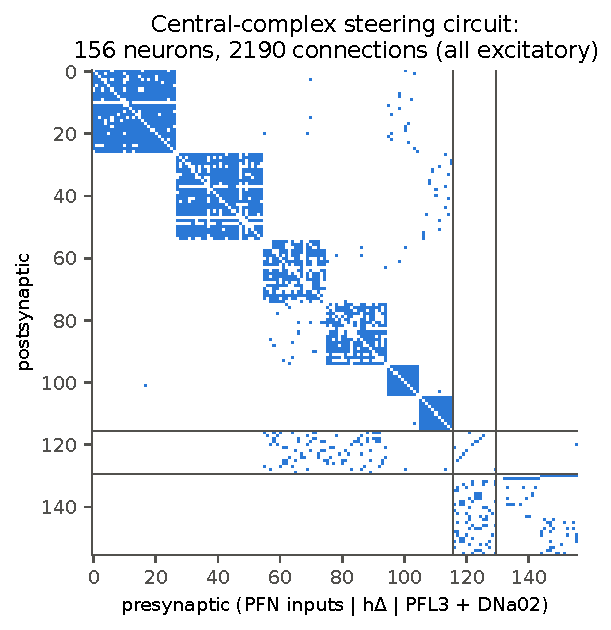
\includegraphics[width=0.40\linewidth]{../figures/fig1_circuit.pdf}\hfill
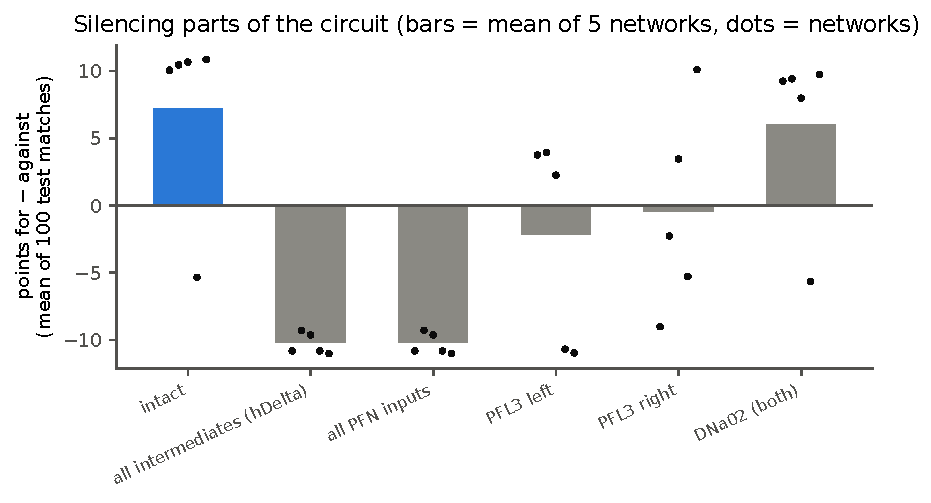
\includegraphics[width=0.57\linewidth]{../figures/fig4_lesion.pdf}
\caption{Left: the extracted steering pathway (PFN inputs, h$\Delta$ intermediates, PFL3 and DNa02
outputs; all connections excitatory). Right: point difference per match after silencing a group of
cells; dots are the five trained networks.}
\label{fig:circuit}
\end{figure}

\section{Results}
Every test match was won in four of the five runs, with between \GoodAgainstMin{} and
\GoodAgainstMax{} points conceded per match and at least \GoodReturnMin\% of incoming balls returned
(Table~\ref{tab:seeds}). Unlike the ball-following rule, points are also scored by these agents, most
plausibly through returns placed at angles the slow opponent cannot reach, although shot angles were
not analysed. A weaker solution was reached in run \BadSeed{} (\BadFor{}--\BadAgainst{}, \BadWinPct\%
wins), which is still far above a motionless paddle. The tracking of the ball by the paddle over
several rallies is shown in Fig.~\ref{fig:rally}.

\begin{table}[t]
\centering\small
\caption{Test performance per run (100 matches each).}
\label{tab:seeds}
\begin{tabular}{rrrrrr}
\toprule
seed & points & match wins & returns per match & return rate & training (s) \\
\midrule
\SeedRows
\bottomrule
\end{tabular}
\end{table}

Silencing is more consequential here than the size of the circuit suggests. When the
\Intermediates{} h$\Delta$ cells were removed, all matches were lost in every run (at most
\MidLesForMax{} points), exactly as when all PFN inputs were removed; this is expected from the
absence of direct input--output connections. In contrast, some runs were left almost intact and
others were broken when the PFL3 cells of one hemisphere were removed, and the removal of both DNa02
cells was mostly harmless. The learned interfaces therefore depend on the measured multisynaptic
route, but the output population is used differently from run to run.

\begin{figure}[t]
\centering
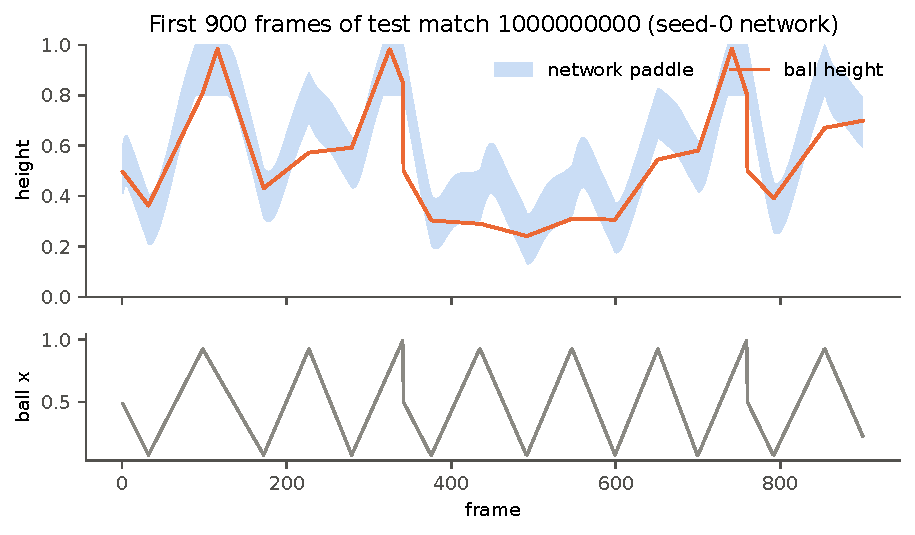
\includegraphics[width=0.95\linewidth]{../figures/fig3_rally.pdf}
\caption{Ball height with the paddle's extent (top) and ball horizontal position (bottom) over the
first 900 frames of a test match.}
\label{fig:rally}
\end{figure}

\section{Discussion}
A frozen central-complex pathway can serve as the controller of a one-dimensional tracking task, and
the signal demonstrably passes through its interneurons. The result is bounded by three caveats. The
opponent is weak by construction and the ball state is handed to the agent by the readings, so the
circuit is not probed deeply by the task. Matched random graphs were not tested, so no advantage of
the measured wiring is claimed; the informative comparison here is internal, between circuit parts.
Finally, the readout episode is a reminder that results of this kind are partly a property of the
interface: the same frozen circuit was useless or effective depending on how its output cells were
pooled, which cautions against reading biological meaning into the success of such mappings. The
variability across runs, with one of five failing, points the same way.

\section{Conclusion}
With its weights untouched, a \Neurons{}-neuron steering pathway from the FlyWire connectome plays
Pong well in four of five independent optimisations, and the ability is lost entirely when its
h$\Delta$ interneurons are silenced.

\paragraph{Data and code availability.} Connectivity and transmitter predictions were downloaded
from the FlyWire Codex portal (v783) \cite{dorkenwald2024}. All scripts, per-run logs and the demo
page are hosted at \url{https://github.com/burakgulmez/fly-pong}.

\bibliographystyle{plain}
\bibliography{refs}
\end{document}
